\section{网络架构}

\begin{figure}[htbp]
    \centering
    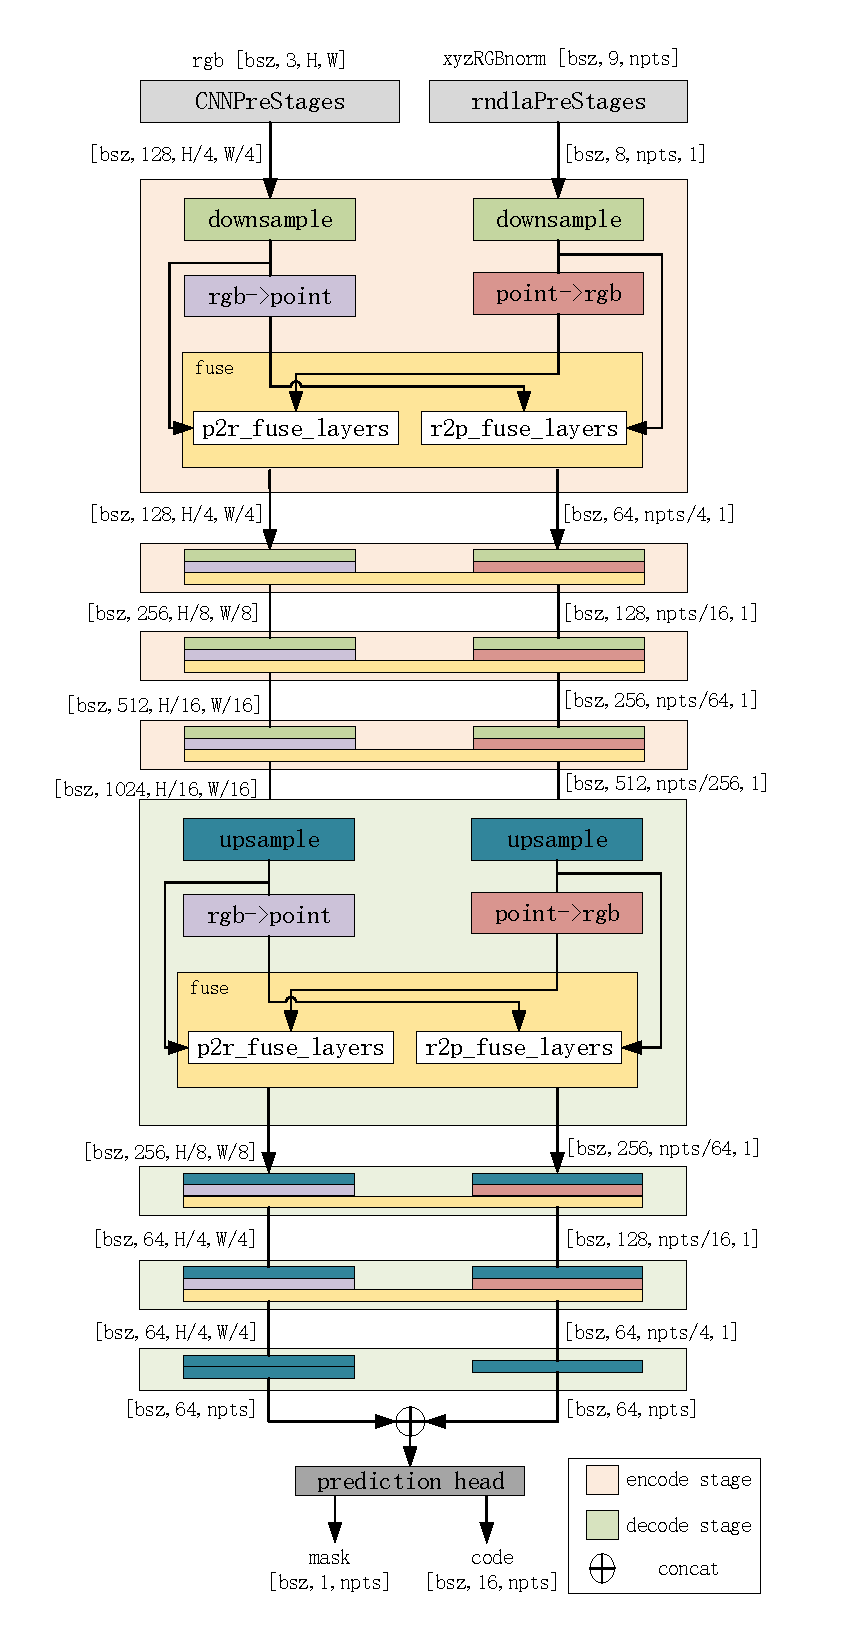
\includegraphics[width=0.68\textwidth]{figure/hipose/network.pdf}
    \caption{网络架构}
    \label{fig:detail_network}
\end{figure}

\autoref{fig:detail_network}展示HiPose的网络结构,其包含两个分支:RGB分支和点云分支。网络包含四个编码器块和四个解码器块。除了最后一个解码器块,每个块执行输入的上采样或下采样,然后处理RGB和点特征,随后将它们合并为一个特征,。在RGB图像分支中,我们采用ConvNeXt\cite{Liu2022ACF}作为编码器,采用PSPNet块\cite{zhao2017pyramid}作为解码器。对于点云分支,我们使用来自Randla\cite{hu2020randla}的模块。图中'bsz'指的是批量大小,'npts'表示点的数量,'H/W'代表图像的高度和宽度。在RGB分支的预处理阶段(CNNPreStages),尺寸为$3 \times H \times W$的裁剪图像被转换为尺寸为$128 \times H/4 \times W/4$的RGB特征。其中,$H$和$W$分别表示输入裁剪RGB图像的高度和宽度,默认情况下均设置为256。另一方面,点云分支的与处理阶段(rndlaPreStages)之前,输入为点坐标、RGB颜色和法线方向拼接成长度为9的点特征。参数$npts$表示有效输入点云的数量,默认设置为2730。若观测点云数量不足$npts$,则会复制补齐,若输入点云数量超过$npts$,则会进行随机采样。两个分支都由相互连接的编码器和解码器构成,主要用于特征提取、特征转换和特征融合。

特征提取过程旨在提取语义特征并为了完成网络级联而调整通道维度。我们采用RandLA-Net~\cite{hu2020randla}来处理点云特征。此外,预训练的ConvNeXt-B\cite{Liu2022ACF}和PSPNet\cite{zhao2017pyramid}模型被集成到编码器和解码器模块中。

特征转换过程是指通过坐标对应关系在RGB分支和点云分支之间进行特征转换。具体而言,如\autoref{fig:p2r_r2p}所示,点云分支的特征可以通过聚合RGB分支中最近的特征来生成。同样,RGB分支的特征可以通过插值点云分支的特征来生成。这实现了RGB分支和点云分支特征之间的双向转换。\autoref{fig:p2r_r2p}上方的模块表示将RGB特征转换为点特征,记作$r2p\_emb$,而下方的模块表示将点特征转换为RGB特征,记作$p2r\_emb$。$r2p\_neighbor\_index$表示每个点特征对应的最近像素的索引,$p2r\_neighbor\_index$同理。

\begin{figure}[htbp]
    \centering
    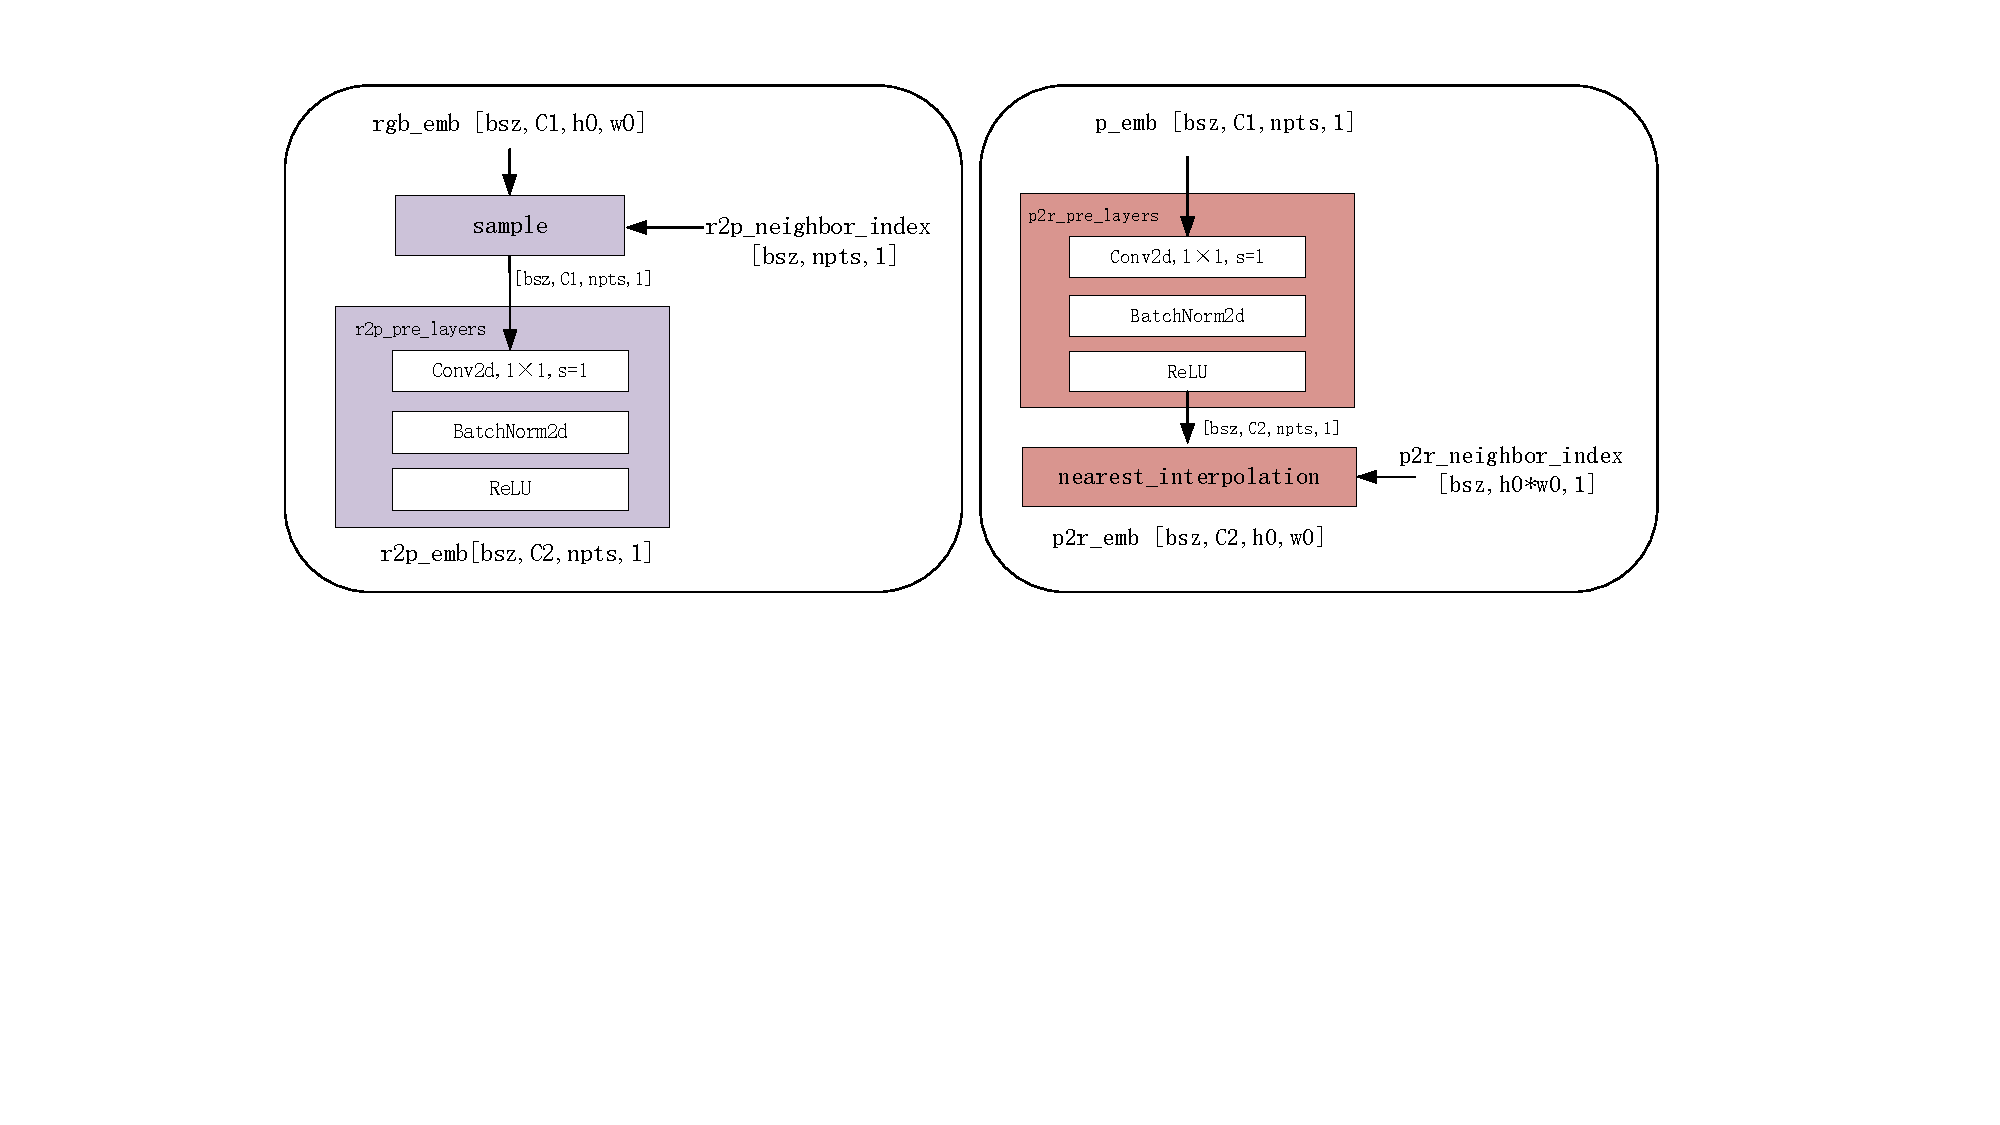
\includegraphics[width=0.5\textwidth]{figure/hipose/p2r_r2p.pdf}
    \caption{特征转换模块}
    \label{fig:p2r_r2p}
\end{figure}

特征融合过程是通过卷积神经网络(CNN)执行的。新的RGB特征是通过将RGB特征与转换后的RGB特征连接生成的,深度特征的处理过程也是如此。有关特征融合过程的更多细节可以在\autoref{fig:fuse}中看到。我中,(a) 表示融合模块的特征流向。(b) 模块用于融合RGB特征 $rgb\_emb$ 和点到RGB特征 $p2r\_emb$。(c) 模块负责融合点特征 $p_emb$ 和RGB到点特征 $r2p\_emb$。

\begin{figure}[htbp]
    \centering
    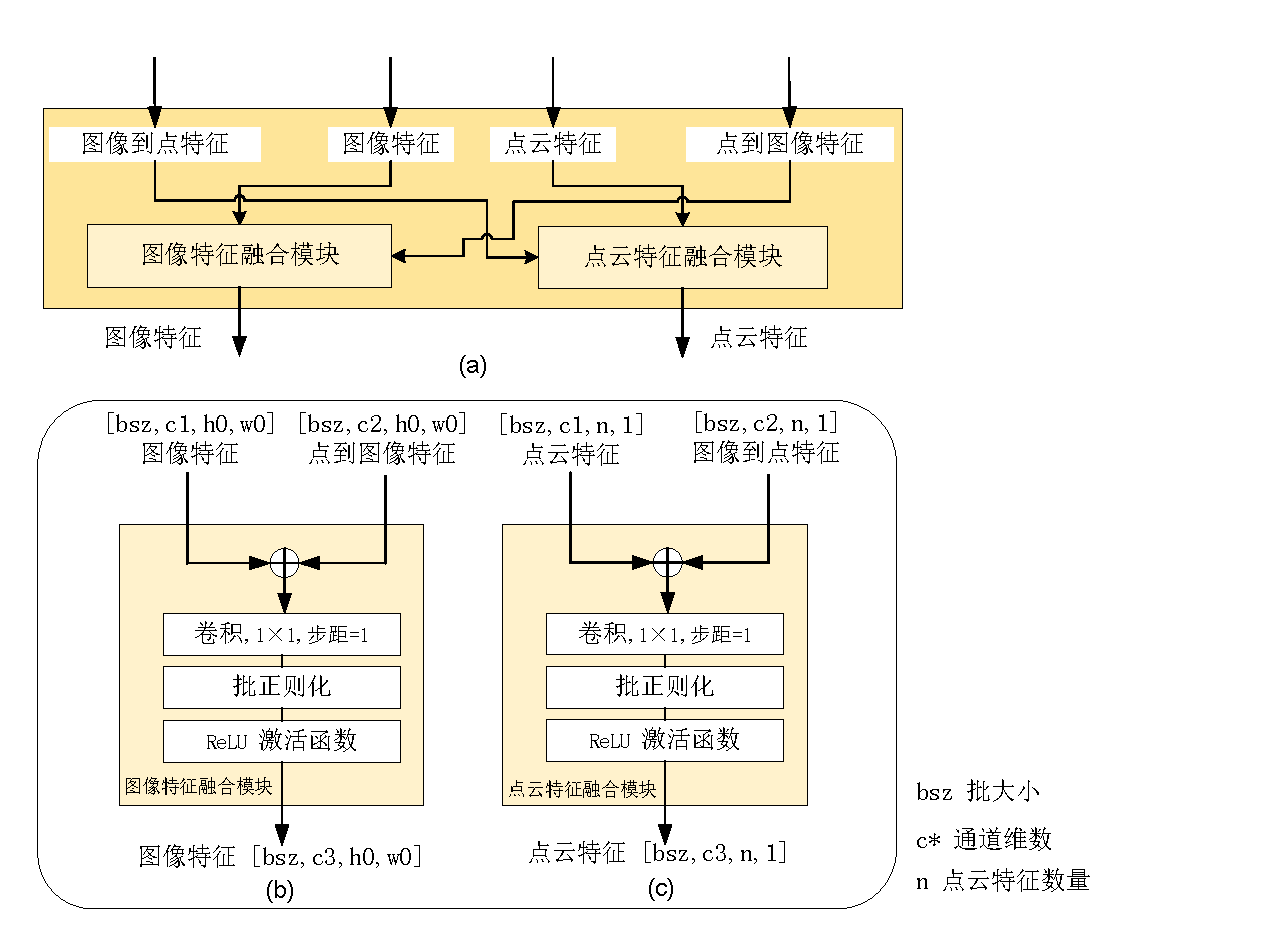
\includegraphics[width=0.5\textwidth]{figure/hipose/fuse.pdf}
    \caption{特征融合模块}
    \label{fig:fuse}
\end{figure}


最后,我们使用一个基于卷积的网络头(head)来预测所选$npts$点的可见掩码和编码。其中编码长度为16位。

\subsection{实现细节}\label{subsection:implementation_details}
本章方法可以便捷地集成到各种现有的RGB-D网络中。本章以FFB6D\cite{he2021ffb6d}的全流双向融合网络为基础,进行了一些修改,构建了HiPose网络。

与FFB6D类似,我们的HiPose网络也有两个分支,分别处理图像和点云。我们将(1) 放大后的物体区域(RoI)图像和(2)从RoI深度图中均匀采样固定数量像素生成的点云输入到HiPose网络中。
我们还对输出层进行了修改。我们将三个输出头替换为一个包含可见性掩码和每个随机选择点的长度为 $d$ 的二进制编码的单一输出头。可见性掩码和二进制编码都使用 L1 损失。训练损失(Loss)定义为
\begin{equation}
Loss = L_{mask} + \alpha L_{code}   
\end{equation}
其中 $\alpha$ 是掩码和二进制编码损失之间的权重因子,在所有实验中设置为 $\alpha = 3$。对于二进制编码预测,我们只计算预测可见掩码内点的损失。

对于网络骨干(backbone),我们使用ConvNext\cite{Liu2022ACF}架构,该架构基于ResNet\cite{He2015DeepRL}。ConvNext在性能上与Vision Transformer\cite{Dosovitskiy2020AnII}相当,同时保留了ResNet的效率和简洁性。

我们将网络训练了$38$万次迭代(batch size),批量大小为$32$。我们使用Adam\cite{Kingma2014AdamAM}优化器,固定学习率为$1e-4$。在训练过程中,我们对RGB图像采用了ZebraPose\cite{su2022zebrapose}中使用的图像数据增强方法,对深度图采用了MegaPose\cite{Labbe2022MegaPose6P}中的深度数据增强方法。
